\documentclass{article}
\usepackage[utf8]{inputenc}
\usepackage[english]{babel}
\usepackage[margin=1in]{geometry}
\setlength{\parindent}{0}
\usepackage[T1]{fontenc} % optional
\renewcommand{\labelenumi}{\alph{enumi}.}

\usepackage{mathtools}
\usepackage{listings}
\usepackage{caption}

\usepackage{color} %red, green, blue, yellow, cyan, magenta, black, white
\definecolor{mygreen}{RGB}{28,172,0} % color values Red, Green, Blue
\definecolor{mylilas}{RGB}{170,55,241}
\definecolor{vblue}{RGB}{49,49,255}
\setlength{\parskip}{1em}

\lstset{language=Matlab,%
    basicstyle=\footnotesize\ttfamily,breaklines=true,
    breaklines=true,%
    morekeywords={matlab2tikz},
    keywordstyle=\color{vblue},%
    morekeywords=[2]{1}, keywordstyle=[2]{\color{black}},
    identifierstyle=\color{black},%
    stringstyle=\color{mylilas},
    commentstyle=\color{mygreen},%
    showstringspaces=false,%without this there will be a symbol in the places where there is a space
    numbers=left,%
    numberstyle={\tiny \color{black}},% size of the numbers
    numbersep=9pt, % this defines how far the numbers are from the text
    emph=[1]{for,end,break},emphstyle=[1]\color{red}, %some words to emphasise
    %emph=[2]{word1,word2}, emphstyle=[2]{style},    
}
 \usepackage[nohead, nomarginpar, margin=1in, foot=.25in]{geometry}

\usepackage{graphicx}
\usepackage[style=apa, backend=biber]{biblatex}
\DeclareLanguageMapping{english}{english-apa}
\addbibresource{bib_test.bib}
\title{Labratory 5\\ ENGR 461: Digital Communications} % Title

\author{Graeme \textsc{Paul}} % Author name

\date{\today} % Date for the report


\begin{document}

\maketitle
\section{Introduction}
In this lab a image is being transmitted within MATLAB. The image is transmitted using 4-PAM modulation. Multiple MATLAB functions were used to implement the transmission. 4-PAM modulation is a method of modulation which uses the amplitude during a pulse to send information. 4-PAM has four different levels of amplitude and can encode two bits per level. The image that is transferred is a 128x128 image. In this lab the transmission is sent through a additive white Gaussian noise channel. The noisy channel can cause error depending on the SNR. The Qfunc is estimated in the lab by finding the BER of the transmission. 
\section{Image Transmission}
\subsubsection{Modulation}
Pulse Amplitude modulation is used to send a signal which contains information through amplitudes sent as pulses. 4-PAM uses four levels of amplitudes which are equally spaced. The amplitudes result in signals which are equally spaced by a distance of $d_{min}$ across the In-Phase axis of the constellation diagram. The distance is dependant on the amplitude of the pulse which is proportional to the energy. The energy of the signal in this lab is set by selecting a desired signal to noise ratio. In this lab SNR is defined as $\frac{\varepsilon_b}{N_o}$.

The desired SNR is first selected then equation 1 can be used to determine $\varepsilon_b$ which is the energy per bit and is entirely dependant on the SNR and Noise $N_o$. The energy per bit then gives average signal energy which can be found with equation 3. The average signal energy then gives d using equation 4. Using equation 5 amplitudes for the modulator can be found from distance. From d the minimum distance between signals can be found to be  $d_{min} = 2d$.
\begin{equation}
    \varepsilon_{b} = N_0 \times 10^{ \frac{ \text{SNR}}{10} }
\end{equation}
\begin{equation}
    \text{SNR} = 10\text{log}_{10}(\frac{\varepsilon_{b}}{N_0}) 
\end{equation}
\begin{equation}
    \varepsilon_{s} = \varepsilon_{b}\text{log}_2(M) 
\end{equation}
\begin{equation}
    d = \sqrt{\frac{3 \varepsilon_{s}}{M^2 - 1}} 
\end{equation}
\begin{equation}
    A_m = (2m - 1 - M)d, m = 1,2, \dots, M
\end{equation}
\begin{center}

\end{center}
In MATLAB the modulator was implemented as a function using the amplitudes found from equation 5 and mapped according to grey coding. Grey coding encodes the bits so that only one bit changes between adjacent levels. The modulator function takes two bits as inputs then uses the grey coding mapping to decide which of the four amplitudes to send the bits as. The encoding scheme is shown in table 1. The constellation diagram for the encoding scheme can be seen in figure 1 below where the circles are the modulated signals with a unit energy, $\varepsilon_s = 1$.
\begin{center}
\captionof{table}{Grey Mapped Modulated Signal Table}

\begin{tabular}{|l|l|l|} \hline
Bits & Modulated Amplitude of Signal as Distance  \\ \hline
00   & -3d\\ \hline
01   & -d     \\ \hline
11   & d  \\ \hline
10   & 3d      \\ \hline
\end{tabular}
\end{center}
\begin{figure}[!h]
        \centering 	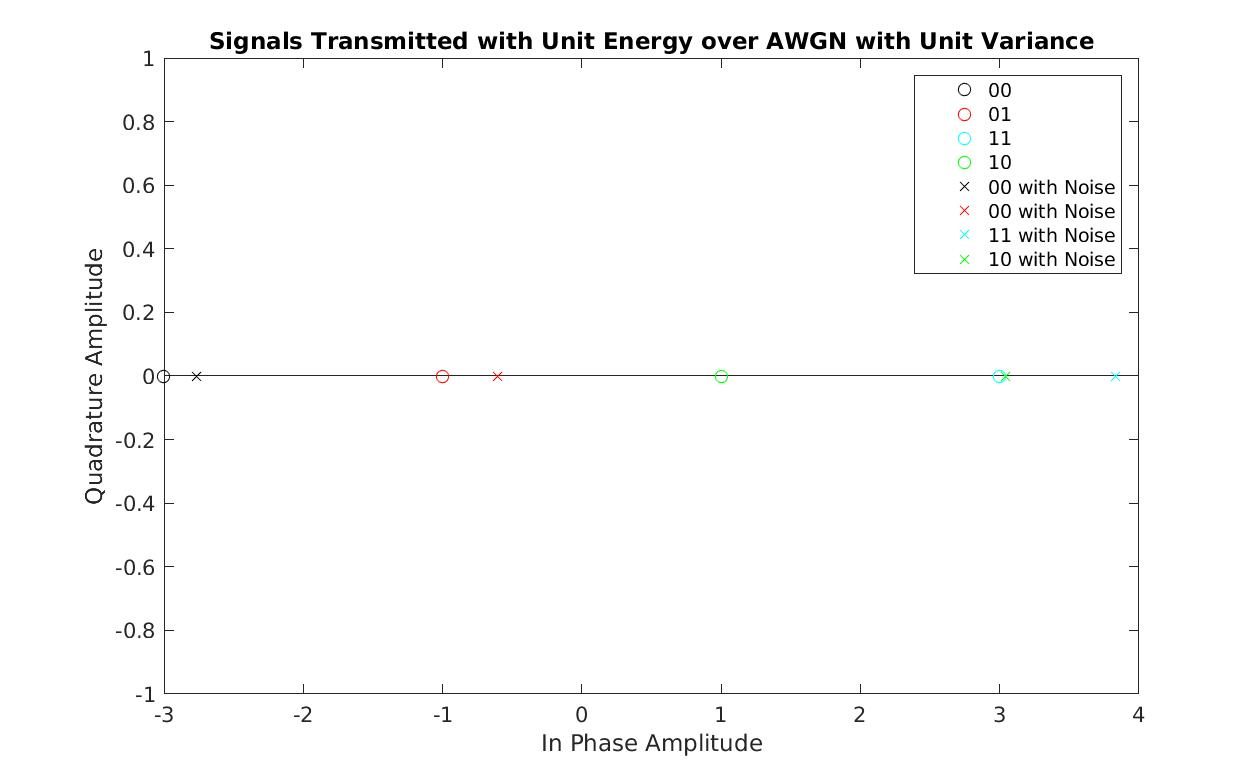
\includegraphics[width=.8\linewidth]{signalconst.jpg}
    \caption{Signal Constellation for 4-PAM modulation}
\end{figure}
\subsection{Channel Noise}
In this lab the image is transmitted over a noisy channel. The noise of the channel is determined by equation 6 which is the temperature times the Boltzmann constant. This models thermal noise that would exist in a channel. With this value determined the signal to noise ratio can be determined using equation 2. When the modulated signal passes through the channel the noise is added to the modulated signal. The channel is a additive white Gaussian noise channel so the noise added to the signal and is zero mean Gaussian noise. The noise will cause the signal to shift left or right on the signal constellations. The noise + signal are plotted on the signal constellation in figure 1 as an X, in this plot the noise is zero mean unit variance causing the signal to move left or right.
\begin{equation}
    N_0 = k_bT = 1.38 \times 10 ^{-23} \frac{J}{K} \times 300K = 4.1400 \times 10^{-21} J
\end{equation}
\subsubsection{Demodulation}
After passing through the channel demodulation occurs. Demodulation takes the signal values and uses them to retrieve the original information. The demodulator uses a decision region which is optimal for equiprobable signal transmission, shown in the table below. These values were found from equation 4 knowing that the distance between two signals is $d_{min} = 2d$.
\begin{center}
\captionof{table}{Grey Mapped Modulated Signal Table and Decision Region}
\begin{tabular}{|l|l|l|} \hline
Bits & Modulated Amplitude of Signal          & Decision Region \\ \hline
00   & -3d     & $y \leq -2d$	  \\ \hline
01   & -d     & $-2d < y \leq 0$    \\ \hline
11   & d     & $0 < y \leq 2d$     \\ \hline
10   & 3d      & $y \geq 2d$     \\ \hline
\end{tabular}
\end{center}

\subsection{Bit Error Rate}
The bit error rate can be calculated using equation 4, and the symbol error rate can be calculated using equation 5. Both the symbol error rate and the bit error rate were used to analyze the performance of the codes at various SNR.
\begin{equation}
    \text{Bit Error Rate} = \frac{\text{Number of Bit Errors}}{\text{Number of Bits Transmitted}}
\end{equation}
\begin{equation}
    \text{Symbol Error Rate} = \frac{\text{Number of Symbol Errors}}{\text{Number of Symbols Transmitted}}
\end{equation}
\begin{equation}
    \text{SER}_{\text{4PAM}}^{\text{AWGN}} = 2(1-\frac{1}{M})Q(\frac{d}{\sqrt{No/2}});
\end{equation}
\section{Results}
In the first part of the lab 4PAM was used to modulate a signal with a unit signal energy $\varepsilon_s = 1$. Using equation 4 the required distance can be found. This was then added to noise with zero mean and unit variance. The result is seen in figure 2, which is a copy of figure 1. The signals without noise are circles and the signals with the added noise are shown as an X.
\begin{figure}[!h]
        \centering 	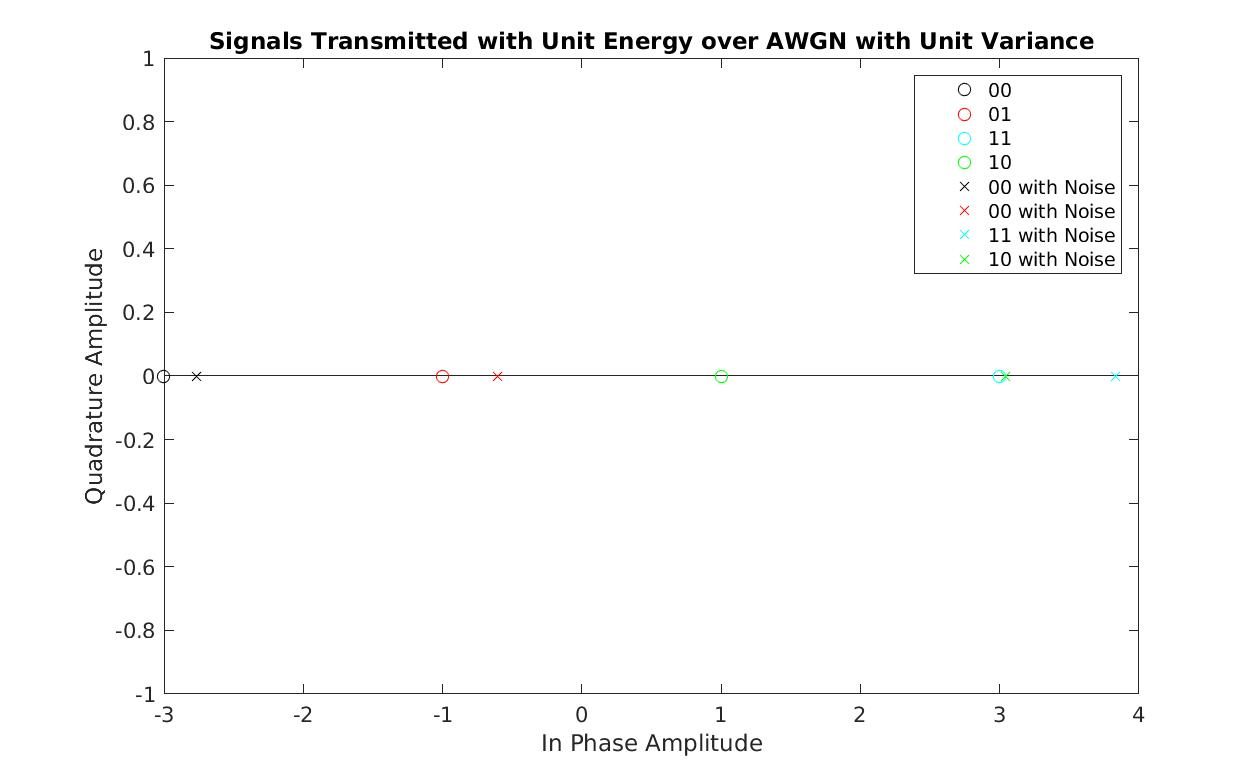
\includegraphics[width=.8\linewidth]{signalconst.jpg}
    \caption{Signal Constellation for 4-PAM modulation}
\end{figure}
\clearpage

The image lena128.jpg was then sent using 4PAM transmission at various bit energy SNRs 
(SNR = $\frac{\varepsilon_b}{N_o}$ = 0:1:10). This was done first by using equation 1 to find $\varepsilon_b$ for a given SNR then using equation 3 and 4 to find d, which is then used to give amplitudes with equation 5. 

It can be seen from the table below that the when the SNR ($\frac{\varepsilon_b}{N_o}$) is increased the number of errors decreases. This characteristic can also be seen in figure 2 where 4-PAM estimated BER and 2-PAM theoretical and estimated BER are plotted. The graph shows the decreasing nature of BER as SNR is increased. When compared to 2-PAM it can be seen that 4-PAM has greater number of errors. Therefore at equal bit energies 2-PAM performs better than 4-PAM for signal integrity. This is due to the minimum distance of 4-PAM which is less than that of 2-PAM for equal bit energies which can be seen in equation 13 and equation 14. This causes the decision region to reduce and therefore noise is more likely to cause bit errors. In addition signals $s_2$ and $s_3$ have smaller decision regions as they are both adjacent to other signals, where as in 2-PAM both signals have decision regions which go from 0 to +/-$\infty$. In addition the BER could be further increased by large spikes of noise or with bad encoding as there is also a possibility that two bit errors occur per symbol error which can also increase the number of bit errors. These three effects add up together causing 4-PAM to have more errors than 2-PAM at equal SNR ($\frac{\varepsilon_b}{N_o}$). 

Using Q-func the SER for 4-PAM can be calculated using equation 11. It is plotted along with the estimated SER for the transmitted image in figure 4 and can be seen to be very close. The percent error between the two can be seen in figure 5, which shows that the two are very close. This shows that estimating the SER for 4PAM by counting the number of symbol errors is a good estimate for Qfunc.

The reconstructed images are shown in figure 6 and figure 7. It can be seen visually that 2-PAM performs better than 4-PAM at the same SNR ($\frac{\varepsilon_b}{N_o}$). These images also show how the BER reduces as the SNR increases.

If a BER of $10^{-2}$ was required to transmit the image then different SNRs ($\frac{\varepsilon_b}{N_o}$) would need to be used for 4-PAM and 2-PAM. Where $-20dB = 10\text{log}(10^{-2})$, the graph can be used to find the SNR that is needed. It can be seen that 2-PAM line crosses -20dB line at about 4.2SNR($\frac{\varepsilon_b}{N_o}$) and the 4-PAM line crosses -20dB at around 7.8dBSNR($\frac{\varepsilon_b}{N_o}$). The table also aligns with these estimates showing for 2-PAM it is between 4 and 5 SNR and for 4-PAM it is between 7 and 8 SNR. Therefore this test shows that 4-PAM requires more energy per bit to transmit at the same error rate as 2-PAM. 


\begin{equation}
    \text{BER}_{\text{2PAM}}^{\text{AWGN}} = Q(\sqrt{\frac{\varepsilon_{b}}{N_0}})
\end{equation}
\begin{equation}
    \text{SER}_{\text{4PAM}}^{\text{AWGN}} = (1.5)Q(\frac{d}{\sqrt{No/2}});
\end{equation}
\begin{equation}
   d_{min,MPAM} = 2 * d = 2( \sqrt{3 \frac{\varepsilon_s}{M^2 - 1}})
\end{equation}
\begin{equation}
   d_{min,2PAM} = 2 * d = 2\sqrt{\varepsilon_b}
\end{equation}
\begin{equation}
   d_{min,4PAM} = 2 * d = 2\sqrt{\frac{2\varepsilon_b}{5}}
\end{equation}
\newpage
\begin{center}
\captionof{table}{Estimated BER for 2-PAM and 4-PAM} 
\begin{tabular}{|l|l|l|l|l|} \hline
SNR ($\frac{\varepsilon_b}{N_o}$)dB & BER4     & BER2     & Errors 4PAM & Error 2PAM \\ \hline
0   & 0.142924 & 7.88E-02 & 56200       & 30985   \\ \hline
1   & 0.120425 & 5.59E-02 & 47353       & 21994   \\ \hline
2   & 0.098946 & 3.73E-02 & 38906    & 14670   \\ \hline
3   & 0.078557 & 2.27E-02 & 30890    & 8909   \\ \hline
4   & 0.059682 & 1.23E-02 & 23468       & 4845   \\ \hline
5   & 0.042699 & 6.00E-03 & 16790    & 2358   \\ \hline
6   & 0.028142 & 2.34E-03 & 11066       & 922   \\ \hline
7   & 0.017293 & 7.22E-04 & 6800    & 284   \\ \hline
8   & 0.009196 & 1.83E-04 & 3615    & 72   \\ \hline
9   & 0.004407 & 2.80E-05 & 1733    & 10   \\ \hline
10  & 0.001775 & 1.02E-05 & 697    & 4   \\ \hline
\end{tabular}
\end{center}
\newpage
\begin{figure}
        \centering 	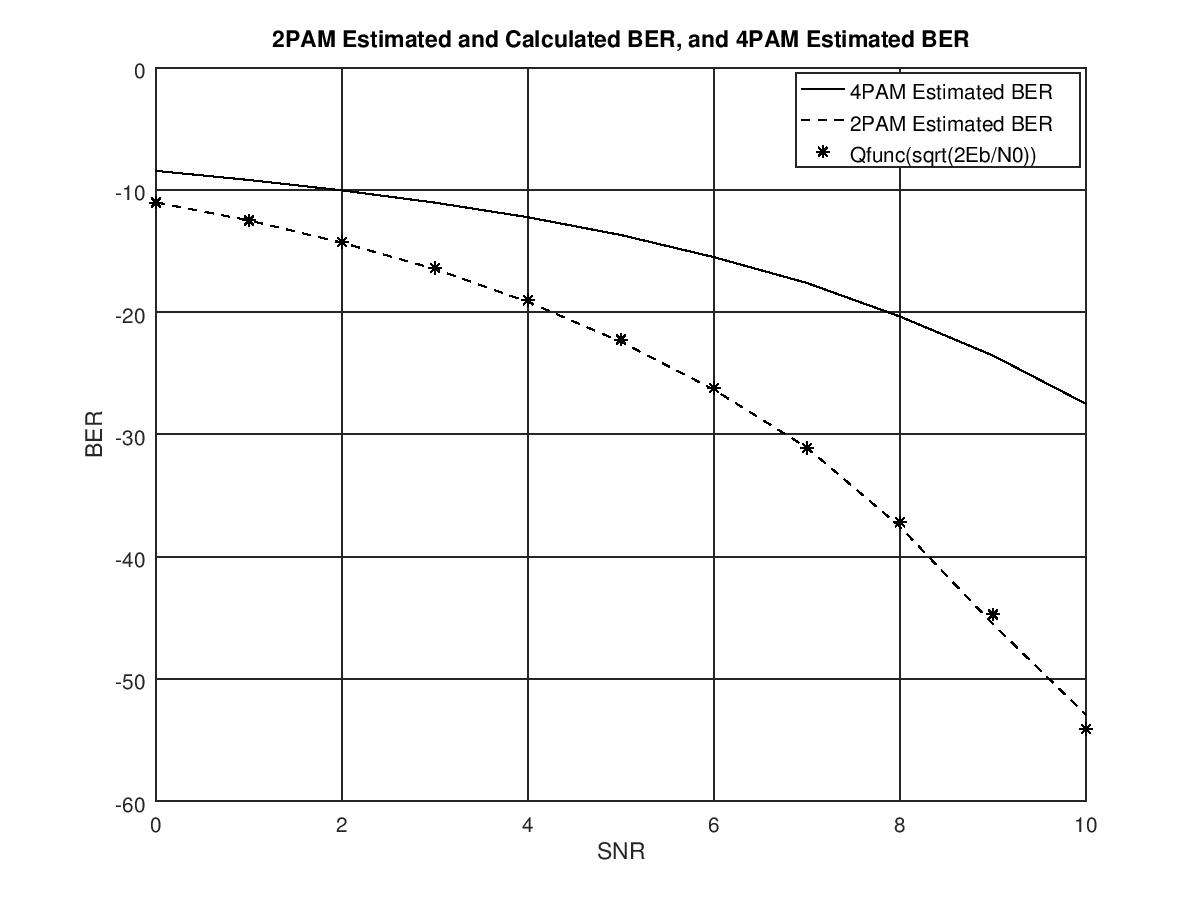
\includegraphics[width=\linewidth]{2pam2pam4pam.jpg}
    \caption{2-PAM Calculated BER and Estimated and 4-PAM Estimated BER, with Grid}
\end{figure}
\begin{figure}
        \centering 	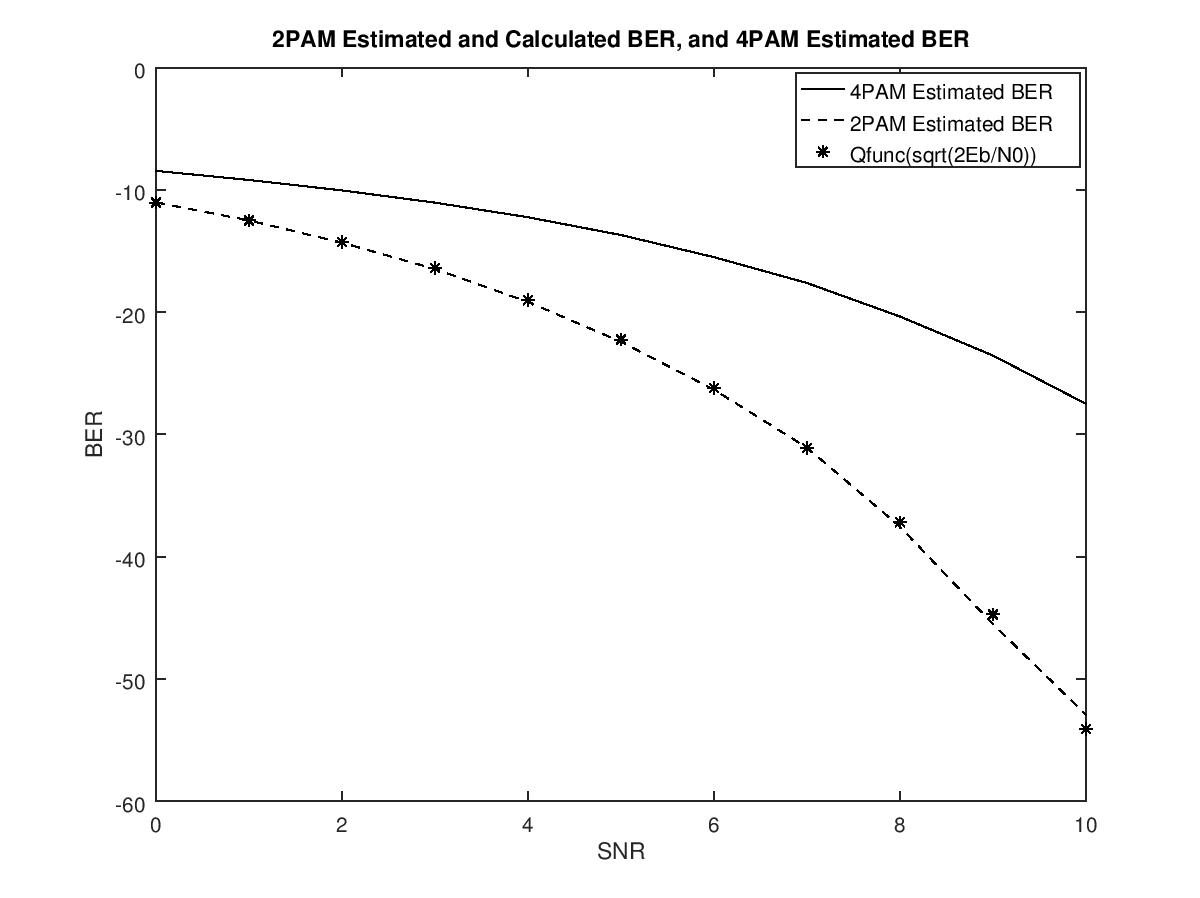
\includegraphics[width=\linewidth]{2pam2pam4pam_nogrid.jpg}
    \caption{2-PAM Calculated BER and Estimated and 4-PAM Estimated BER, without Grid}
\end{figure}
\begin{figure}
        \centering 	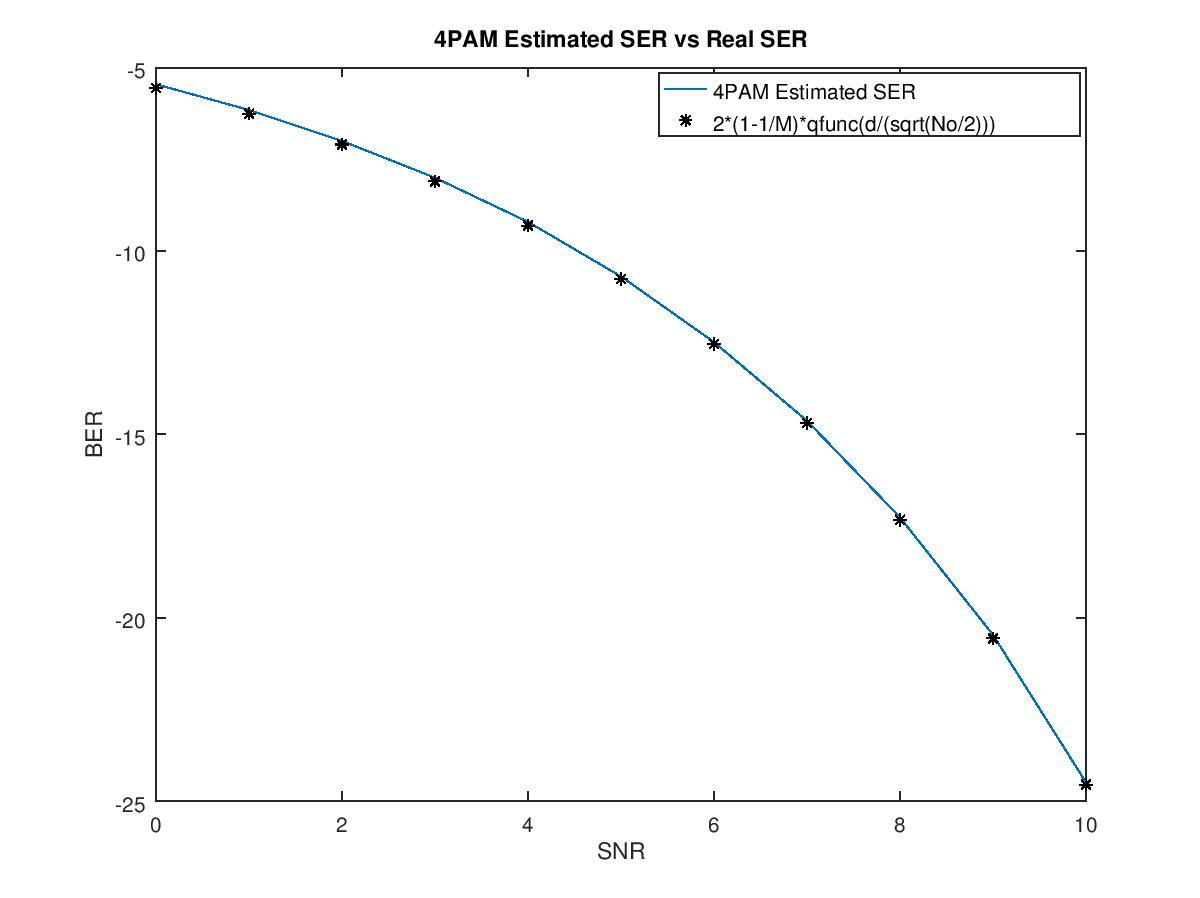
\includegraphics[width=\linewidth]{4pamser.jpg}
    \caption{4-PAM Estimated SER and 4-PAM Calculated SER}
\end{figure}
\begin{figure}
        \centering 	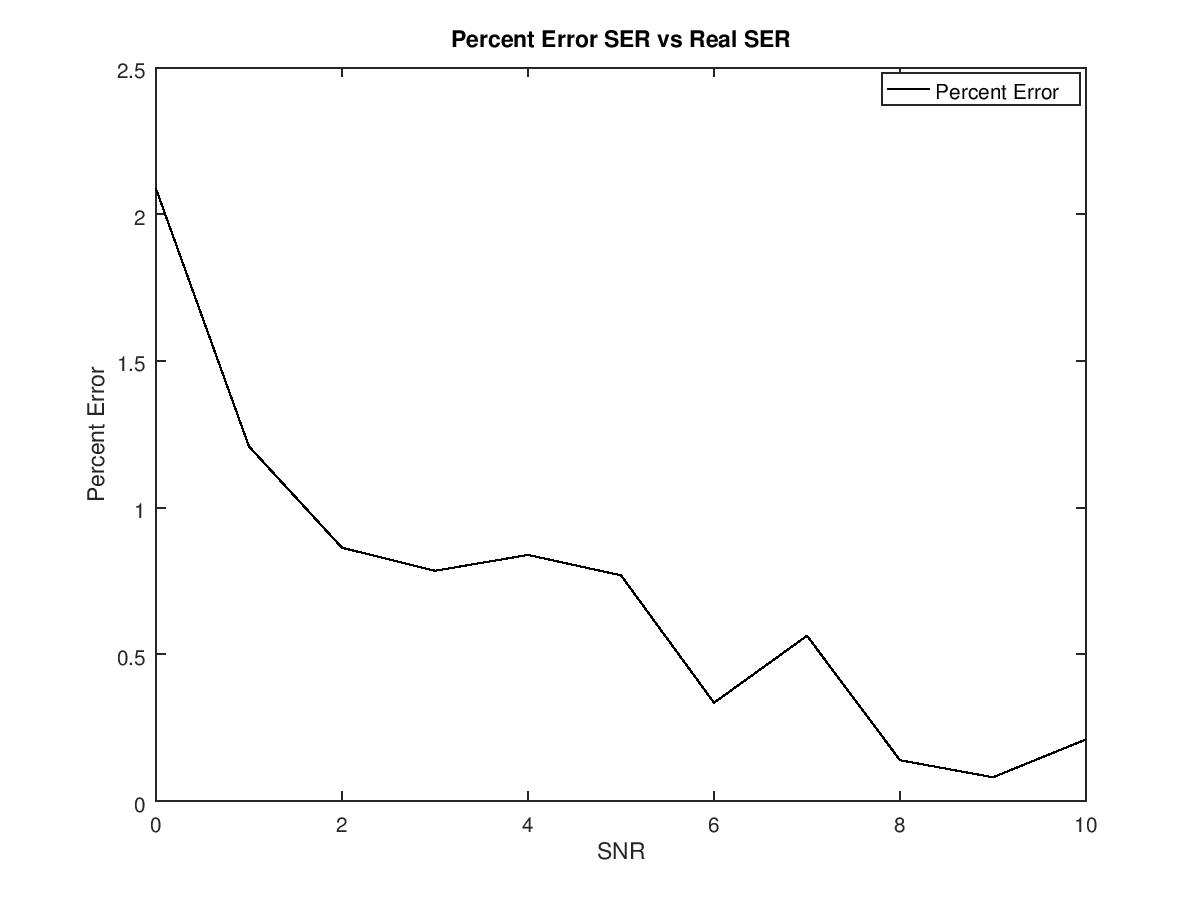
\includegraphics[width=\linewidth]{errorser.jpg}
    \caption{4-PAM Estimated SER Error}
\end{figure}
\newpage
\clearpage
\begin{figure}
        \centering 	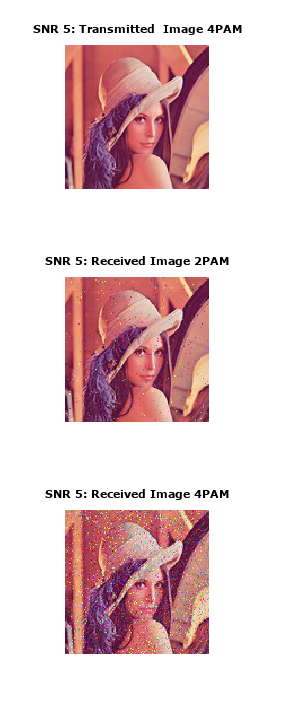
\includegraphics[width=.2\linewidth]{lena5.PNG}
    \caption{Received and Transmitted Images of SNR 5 channel}
\end{figure}
\newpage
\begin{figure}
        \centering 	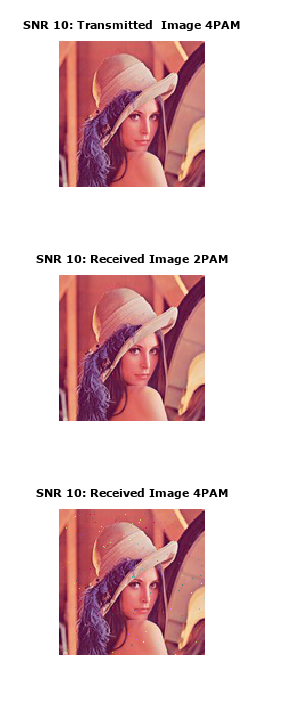
\includegraphics[width=.2\linewidth]{lena10.PNG}
    \caption{Received and Transmitted Images of SNR 10 channel}
\end{figure}
\clearpage
\section{Conclusion}
In this lab a image was transmitted in MATLAB using 4-PAM. The image was transmitted over a additive white Gaussian noise channel with various SNRs. Two functions were created to modulate and demodulate the image using 4-PAM. Grey coding was used to encode the bits to four different amplitudes. To demodulate a decision region for equiprobable signal transmission was used and amplitudes were put back to bits. The bit error rate was estimated by finding it across the SNR  range of $\frac{\varepsilon_b}{N_o}$ = 0:1:10 and compared to the bit error rate for 2-PAM found in lab 4. It was found that for the same energy per bit 4-PAM has a higher bit error rate than 2-PAM, which was mostly due to the decreased decision regions that 4-PAM has. From the reconstructed images and the graphs it can be seen that the BER goes down when SNR increases. The estimated SER for 4-PAM was compared to the theoretical from using Qfunc and it was shown that they match. Lastly the BER of $10^{-2}$ was desired and the SNR was found for 4PAM and 2PAM to transmit at this BER. This again showed that to transmit at the same BER 4PAM requires a larger SNR than 2PAM. Overall this lab showed the bit error performance of 4-PAM compared to 2-PAM. 
\newpage

\section{Appendix}
\subsection{MATLAB Code}
\subsection{Modulation}
\lstinputlisting{FourPammodem.m}
\subsection{Demodulation}
\lstinputlisting{FourPamdemodem.m}
\subsection{Lab code}
\lstinputlisting{lab5.m}

\end{document}